\chapter{Overview of Uintah} \label{Sec:Overview} 
The Uintah Computational Framework (also referred to as Uintah or the UCF)
consists of a set of
software components and libraries that facilitate the solution of
Partial Differential Equations (PDEs) on Structured AMR (SAMR) grids
using hundreds to thousands of processors.

One of the challenges in designing a parallel, component-based
and multi-physics application is determining how to efficiently decompose
the problem domain. Components, by definition, make local
decisions. Yet parallel efficiency is only obtained through a globally
optimal domain decomposition and scheduling of computational
tasks. Typical techniques include allocating disjoint sets of
processing resources to each component, or defining a single domain
decomposition that is a compromise between the ideal load balance of
multiple components. However, neither of these techniques will achieve
maximum efficiency for complex multi-physics problems.

Uintah uses a non-traditional approach to achieving parallelism by
employing an abstract task graph representation to describe
computation and communication. The task graph (see
Figure~\ref{fig:TaskGraph}) is an explicit representation of the
computation and communication that occur in the coarse of a single
iteration of the simulation (typically a timestep or nonlinear solver
iteration). Uintah components delegate decisions about parallelism to
a scheduler component by using variable dependencies to describe
communication patterns and characterizing computational workloads to
facilitate a global resource optimization. The task graph
representation has a number of advantages, including efficient
fine-grained coupling of multi-physics components, flexible load
balancing mechanisms and a separation of application concerns from
parallelism concerns. However, it creates a challenge for scalability
which we overcome by creating an implicit definition of this graph and
representing it in a distributed fashion.

%\begin{figure}
%  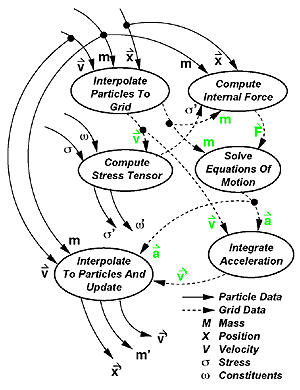
\includegraphics[scale=1]{Taskgraph-diagram.png}
%  \caption{Example Task Graph}
%  \label{fig:TaskGraph}
%\end{figure}

The primary advantage of a component-based approach is that it
facilitates the separate development of simulation algorithms, models,
and infrastructure. Components of the simulation can evolve
independently. The component-based architecture allows pieces of the
system to be implemented in a rudimentary form at first and then
evolve as the technologies mature. Most importantly, Uintah allows the
aspects of parallelism (schedulers, load-balancers, parallel
input/output, and so forth) to evolve independently of the simulation
components. Furthermore, components enable replacement of computation
pieces without complex decision logic in the code itself.

Please see the Developers Guide for more information about the
internal architecture of Uintah.
